\chapter{Literature Study}
% put these two lines after every \chapter{} command
\vspace{-2em}
\minitoc

The implementation of FDIR on satellites have multiple complications with regards to the type of data generated by a satellite and the methodologies that can be implemented within the time and memory constraint of a cube-sat processor.

\section{Anomaly Detection on Satellites}
Various methodologies have been tested on different component of satellites. Therefore a summary of these research articles are provided in this section.

\subsection{Analysis and Prediction of Satellite Anomalies}
\textcite{Wintoft}

\subsection{Agent-based algorithm for fault detection and recovery of gyroscope's drift in small satellite missions}
To ensure that the ADCS of satellites are autonomous every aspect of the control must be able to recover from faults. \textcite{carvajal2017agent} developed an algorithm to evaluate the control of a gyroscope and detect whether drifting exists. If drifting is detected the another algorithm is deployed to ensure the recovery of the gyroscope drift by updating the error state vector.

\subsection{Fault isolation of reaction wheels onboard three-axis controlled in-orbit satellite using ensemble machine learning}
\cite{rahimi2020fault}

\subsection{Fault tolerant control for satellites with four reaction wheels}
\cite{jin2008fault}

\subsection{Innovative Fault Detection, Isolation and Recovery Strategies On-Board Spacecraft: State of the Art and Research Challenges}
\cite{wander2013innovative}

\subsection{Machine learning methods for spacecraft telemetry mining}
\cite{ibrahim2018machine}

\subsection{Machine learning techniques for satellite fault diagnosis}
\cite{ibrahim2020machine}

\section{Statistical Methods}
\subsection{Pearson Correlation}
Vectors of certain sensors are highly correlated. For instance the vector of the earth sensor is highly correlated since the magnitude of the vector remains more or less constant. To detect anomalies the correlation of vectors can be measured and with a specified threshold the correlation can be indicated as a anomaly or nor.

The squared Pearson correlation coefficient (SPCC) for vectors depicted as
\linebreak
\\
\centerline{$a = [a_1, a_2, \ldots, a_L]^T,$}
\linebreak
\centerline{$b = [b_1, b_2, \ldots, b_L]^T,$}
\\
is defined as \cite{benesty2009pearson}
\begin{equation}
	\rho^2 (a,b) = \frac{E^2 (a,b)}{E(a^Ta)E(b^Tb)}.
\end{equation}
The correlation coefficient is proven to be constraint as
\begin{equation}
	0 \leq \rho \leq 1,
\end{equation}
where $\rho = 1$ is perfect linear correlation. 

\subsection{Variance}
Within a sequential data sample of the satellite, the variance of the variables should be within a given threshold if the satellite is in a stable condition. The variance of the data sample is defined as 
\begin{equation}
	S^2 = \frac{\sum(x_i + \bar{x})^2}{n-1}
\end{equation}
where $x$ defines the variable within the dataset.

\subsection{Kalman-Filter}
The Kalman-filter application would require the state-space matrices to be provided in the log file.

\subsection{Multivariate Guassian Distribution}
The assumption that the error of our data is generated with a Guassian distribution with a specific mean, $\mu$, and variance, $\sigma^2$, provides the opportunity for using multi-variate Gaussian distribution to determine the probability of a data-sample within a dataset. 
\begin{equation}
	\label{mean}
	\mu_j = \frac{1}{m} \sum_{i=1}^{m}x_j^{(i)}
\end{equation}

\begin{equation}
	\label{variance}
	\sigma_j^2 = \frac{1}{m} \sum_{i=1}^{m}(x_j^{(i)} - \mu_j)^2
\end{equation}

\begin{equation}
	\label{guassian distribution}
	p(x) = \prod_{j=1}^{n} \frac{1}{\sqrt{2\pi}\sigma_j}exp(-\frac{(x_j-\mu_j)^2}{2\sigma_j^2})
\end{equation}

For multi-variate Guassian distribution \cite{do2008multivariate}.

\begin{equation}
	\label{sum}
	\sum = \frac{1}{m}\sum_{i=1}^{m}(x^{(i)}-\mu)(x^{(i)}-\mu)^T
\end{equation}

\begin{equation}
	\label{multi-variate guassian distribution}
	p(x) = \frac{1}{(2\pi)^{\frac{n}{2}}{\lvert \sum \rvert}^\frac{1}{2}} exp(-\frac{1}{2}(x-\mu)^T{\sum}^{-1}(x-\mu))
\end{equation}

The Anomalies will be classified based on probabilities smaller than a given threshold $p(x) < \epsilon$.

\begin{algorithm}
	\SetKwInOut{Input}{Input}
	\SetKwInOut{Output}{Output}
	
	\SetKwData{Left}{left}
	\SetKwData{This}{this}
	\SetKwData{Up}{up}
	\SetKwFunction{Union}{Union}
	\SetKwFunction{FindCompress}{FindCompress}
	
	\Indm
	\Input{Data sample from satellite orbit.}
	\Output{Whether dataset contains anomaly.}
	\Indp
	\BlankLine
	
	Determine feature vectors $x_i$ \\
	Determine threshold probabilty, $\epsilon$ \\
	Calculate $\mu_j$ with Eq~\ref{mean} \\
	Calculate $\sigma_j$ with Eq~\ref{variance} \\
	Calculate $p(x)$ with Eq~\ref{guassian distribution} \\
	\If{$p(x) < \epsilon$}{Anomaly $= True$}
	\Else{Anomaly $= False$}
	
	\caption[Multi-variate Guassian Distribution]{Multi-variate Guassian Distribution Algorithm}
	\label{alg}
\end{algorithm}

\subsection{Kullback-Leibler Divergence}
The Kullback-Leibler divergence quantifies the difference between two probability density functions, denoted as $p(x)$ and $q(x)$ \cite{hershey2007approximating}. Satellites are systems that are predictable within a time-series. The divergence between two sequential data buffers from the satellite will have a very similar probability distribution. Therefore calculating the difference between two datasets can be used to detect an anomaly based on a given threshold.

The difference between the probability distributions from datasets, $a$ and $b$, in Figure~\ref{Guassian plot} cannot simply be calculated as the difference in the mean or the difference in the variance. To overcome this, the divergence between the two distributions can be calculated. Intuitively a point $x$ with a high probability in the dataset $a$ should have a high probability in the dataset $b$ if the two datasets have a small divergence. 

\pgfmathdeclarefunction{gauss}{3}{%
	\pgfmathparse{1/(#3*sqrt(2*pi))*exp(-((#1-#2)^2)/(2*#3^2))}%
}
\begin{figure}[!h]
	\centering
	\textbf{Difference Between Probability Distributions}
	\begin{tikzpicture}
		\begin{axis}[
			no markers, 
			domain=-3:6, 
			samples=100,
			ymin=0,
			axis lines*=left, 
			xlabel=$x$,
			every axis y label/.style={at=(current axis.above origin),anchor=south},
			every axis x label/.style={at=(current axis.right of origin),anchor=west},
			height=5cm, 
			width=12cm,
			xtick=\empty, 
			ytick=\empty,
			enlargelimits=false, 
			clip=false, 
			axis on top,
			grid = major,
			hide y axis
			]
			
			\addplot [very thick,cyan!50!black] {gauss(x, 3, 1)};
			
			\pgfmathsetmacro\valueA{gauss(3,3,1)}
			\draw [gray] (axis cs:3,0) -- (axis cs:3,\valueA);
			
			\node[below] at (axis cs:3, 0)  {$\mu_p$}; 
			
			\addplot [very thick,red!50!black] {gauss(x, 1.5, 1.5)};
			
			\pgfmathsetmacro\valueB{gauss(1.5,1.5,1.5)}
			\draw [gray] (axis cs:1.5,0) -- (axis cs:1.5,\valueB);
			
			\node[below] at (axis cs:1.5, 0)  {$\mu_q$}; 
		\end{axis}
		
	\end{tikzpicture}
	\caption{Guassian Distributions}
	\label{Guassian plot}
\end{figure}

The divergence can be expressed as 

\begin{equation}
	KL(P\lvert\lvert Q) = \int p(x) \log \left( \frac{q(x)}{p(x)} \right)dx.
\end{equation}

\subsection{Canonical Correlation Analysis}
Due to the orbital nature of satellites there exist a correlation between various sensors. For instance the sun sensor, magnetometer and earth sensor are correlated based on the desired orientation and orbit of the satellite. This correlation might not be of linear nature, but with non-linear correlation methods such as kernel canonical correlation the correlation can be measured.

However, canonical correlation provides the measure of correlation between a multi-dimensional variable with another multi-dimensional variable. Although this seems profitable for satellite fault detection, it will only be applicable for each the comparison between individual sensors. This will indicate the non-linear correlation of the sun sensor with regards to the magnetometer. The problem however, according to \textcite{chen2017fault} is to, determine the appropriate threshold for which to classify a fault. \textcite{chen2017fault} proposed a method for determining the appropriate threshold on page 5, algorithm 1.
\cite{fukumizu2007statistical}
\cite{zhu2017quality}

Python - Pyrcca package

\subsubsection{K-means-based}
\subsubsection{Guassian Mixture Model}
\subsubsection{Just-In-Time-Learning}
\cite{chen2020just}

\section{Feature Extraction}
To 
https://towardsdatascience.com/feature-extraction-techniques-d619b56e31be
\subsection{Prony's Method}
\subsection{Convolutional Networks}
\subsection{Principal Component Analysis}
\cite{choi2005fault}
\cite{ding2010application}
\subsection{Partial Least Square}
\subsection{Independent Component Analysis}
\subsection{Locally Linear Embedding}
\subsection{Linear Discriminant Analysis}
\subsection{Autoencoder}
\subsection{t-Distributed Stochastic Neighbor Embedding}

\section{Supervised Learning}
Supervised learning consists of models that are trained on labelled data. This is not a problem with simulation, but with the real data, it is a problem and to provide tests on the real data to label it must be proficient. If unsupervised learning and statistical methods are not sufficient in their accuracy, a method for labelling the real data must be provided.

\subsection{Random Forests}
\cite{Shi2006, Paul2018, Primartha2018}

\subsection{Long Short Term Memory}
Time-series data: LSTM or DLSTM

\subsection{Support Vector Machines}
Support Vector Machines

\subsection{Naive Bayes}
Naive Bayes

\subsection{K-nearest neighbours}
K-nearest neighbours

\subsection{Artificial Neural Networks}
Artificial Neural Networks

\section{Unsupervised Learning}
Density-based, distance, Clustering

\subsection{Isolation Forests}
This unsupervised learning methods is based on the principle of isolating data points by slicing the data with random conditions \cite{TonyLiu2008}. The data is randomly split into specified sample sizes with a randomly selected dimension and a randomly selected cut-off value. For each sample size the data must be split until each data point within the sample is isolated from all other data points. Training of a single tree is completed when all the data points are isolated and this training must be repeated for all the data samples, however many are predefined. 

The distance measured from the first split the \emph{tree top} to the isolated data point is used to determine whether a data point is anomalous or not \cite{Hariri2021}. The logical reasoning for support of this algorithm is that data points which are non-anomalous will be more closely related and hence have more splits to separate the data points until isolation is achieved. Therefore, the distance from the tree top for non-anomalous data points will be longer than anomalous data points which will have a shorter distance from the tree top. Therefore non-anomalous data points are closer to the \emph{root}. 

Figure~\ref{Figure-Isolation_Forest} demonstrates the splitting of the data points until isolated. Each split or \emph{branch} only splits the data into two groups. After training multiple trees, a single data point is "sent through the forest" and the distance from the tree top for each tree is calculated and the average of all the trees are used to calculated the average distance for the data point. Using a threshold for the distance, the data point is classified as anomalous or not.

\begin{figure}[h!tb]
	\centering
	
	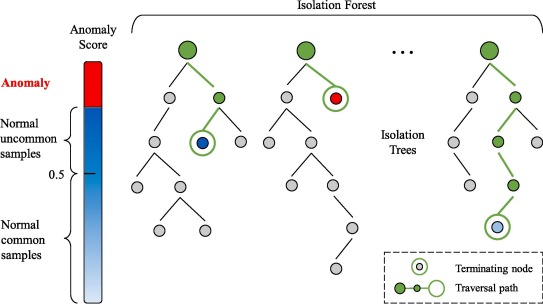
\includegraphics[width=10cm]{fig/Isolation_Forests} % not necessary to give extension - now you can shift between compiling to ps or to pdf without any problems
	
	\caption[Isolation Forest]{Isolation Forests \cite{Chen2020}}
	\label{Figure-Isolation_Forest} 
\end{figure}

The anomaly score is calculated with Eq~\ref{Eq-Isolation_anomaly}
\begin{equation}
s(x,n) = 2^{-E(h(x))/c(n)}
\label{Eq-Isolation_anomaly}
\end{equation}
where $E(h(x))$ is the average value of the distance measured from the tree top for a single data point in all the trees \cite{Hariri2021} and $n$ is the size of a data sample used to train a single tree. For the distance to be normalized, $c(n)$ --- the mean distance from the tree top in an unsuccessful search in a \emph{Binary Search Tree} (BST) --- is used and is calculated as 
\begin{equation}
c(n) = 2H(n-1) - \frac{2(n-1)}{n}.
\label{Eq-normalizing_isolation}
\end{equation}
$H(i)$ in Eq~\ref{Eq-normalizing_isolation} is the harmonic number and is estimated with Euler's constant as 
\begin{equation}
H(i) \approx ln(i) + 0.5772156649.
\label{Eq-H_i}
\end{equation}
Isolation Forests, however have multiple issues, since it splits data in rectangles as seen in Figure~\subref{Figure-ExtendedvsNormal_first}. This is due to the slicing algorithm selecting a feature, $x$ and a cut-off value, $v$. Consequently, the data is either split vertically or horizontally --- if seen as a two dimensional dataset. This split method is unable to categorise complex data structures. These issues however are addressed by \textcite{Hariri2021} and led to the \emph{Extended Isolation Forest} algorithm.

The extended isolation forest algorithm generalises the isolation forest algorithm by applying a slope to each slice. Data points are therefore divided into two groups depending on the "side" of the plane or slice as seen in Figure~\subref{Figure-ExtendedvsNormal_second}.

\begin{figure}[h!tb]
	\centering
	
	\subfloat[][Isolation Forest Slicing example]{
		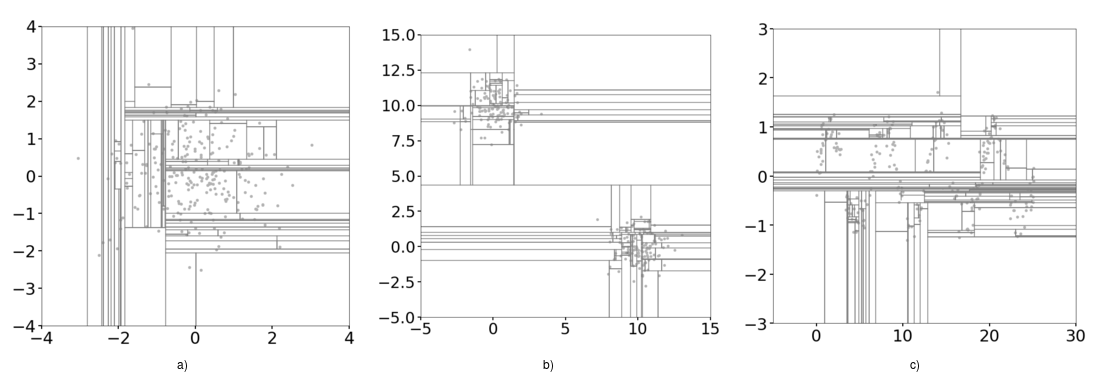
\includegraphics[trim = 0 0 725 0, clip = true, width=7cm]{fig/Isolation_forest_slicing}
		\label{Figure-ExtendedvsNormal_first}
	}
	\quad
	\subfloat[][Extended Isolation Forest Slicing example]{
		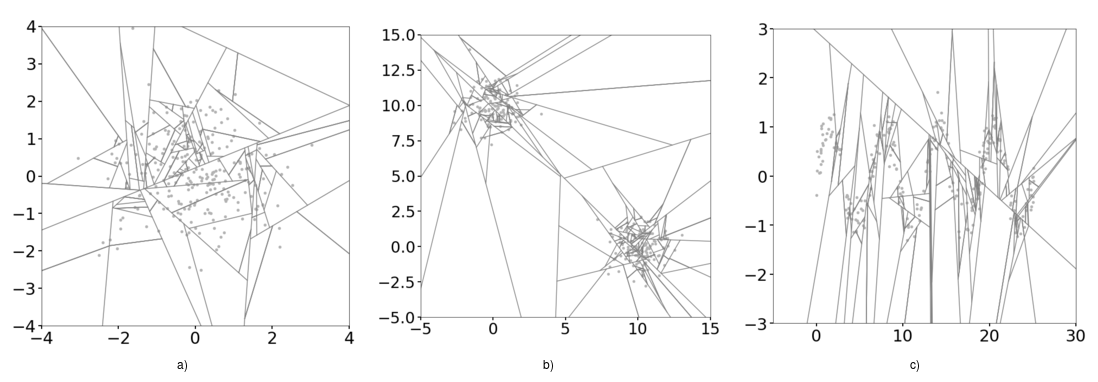
\includegraphics[trim = 0 0 725 0, clip=true,width=7cm]{fig/Extended_Isolation_forest_slicing}
		\label{Figure-ExtendedvsNormal_second}
	}
	\caption[Slicing of Isolation Forest]{The slicing of Isolation Forest vs Extended Isolation Forest}
	\label{Figure-ExtendedvsNormal}
\end{figure}

It is evident that applying an angle of $0\degree$ to all the slices the general algorithm of the extended isolation forest produces the standard isolation forest algorithm where planes or slices are perpendicular to the axis of the randomly selected feature, $x$.

\subsection{Local Outlier Factor}
Most algorithms for anomaly detection are based on a metric which accounts for the entire dataset~\cite{breunig2000lof}. However, many anomalies are identifiable in relation to the local neighbourhood of data points and not the overall dataset. Therefore, \textcite{breunig2000lof} developed the local outlier factor \(LOF\) algorithm that provides a measure of a data point's "outlierness". This implies that a data point is not classified as an anomaly or not, but a local outlier factor is calculated to determine how much a data point is distantiated from it's $k$-nearest neighbours. This is clearly demonstrated in Figure~\ref{Figure-LOF_measure} where the data points which are clustered together have smaller LOF's than data points which are removed from the highly dense areas.

\begin{figure}[h!tb]
	\centering
	
	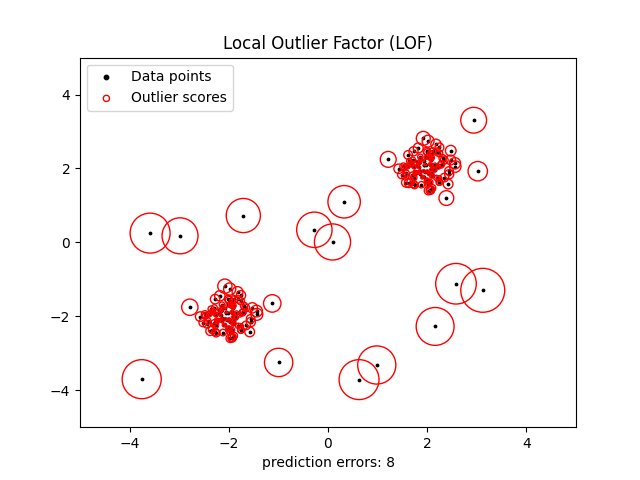
\includegraphics[width=10cm]{fig/LOF_measure} % not necessary to give extension - now you can shift between compiling to ps or to pdf without any problems
	
	\caption[Local outlier measure]{LOF measure}
	\label{Figure-LOF_measure} 
\end{figure}

To calculate the LOF, the $k$-distance must be calculated and also the local reachability density \(lrd\). The $k$-distance, is the $k^{th}$ ranked $distance(o,p_i)$. Where $distance(o,p_i)$ is the distance between data point $o$ and any data point $p_i$, with $i \in N$, where $N$ is the number of data points within the dataset with a minimum value of $MinPts$. To reduce fluctuations in the $distance(o,p_i)$ the distance between $o$ and $p_i$ is replaced with 
\begin{equation}
max \{distance(o,p_i), k\text{-distance}\} 
\end{equation}
and will henceforth be referred to as the reachability distance~\cite{breunig2000lof}. The $lrd$ of a data point, $p$, is calculated as 
\begin{equation}
lrd_{MinPts}(p) = 1/\left(\frac{\sum\limits_{o \in N_{MinPts}(p)}^{} reach\-dist_{MinPts}(p,o)}{|N_{MinPts}(p)|}\right)
\label{Eq-lrd}
\end{equation}
and denotes "the inverse of the average reachability distance based on the $MinPts$-nearest neighbours of the $p$" --- \textcite{breunig2000lof}. Eq~\ref{Eq-lrd} enables the calculation for the $LOF$ of point $p$ as shown in Eq~\ref{Eq-LOF}
\begin{equation}
LOF_{MinPts}(p) = \frac{\sum\limits_{o \in N_{MinPts}(p)}^{}\frac{lrd_{MinPts}(o)}{lrd_{MinPts}(p)}}{|N_{MinPts}(p)|}
\label{Eq-LOF}
\end{equation}
The rule of thumb for detecting an outlier is that when the LOF is larger than 1, then the point is considered an outlier with respect to its neighbourhood. This however is not fixed and the threshold can be changed depending on the application.
 
This method is aimed at producing a measure of the "outlierness" of a data point within a local neighbourhood and not for all the data points. This method will thus be implemented for the satellite anomaly detection, since it will detect anomalies within the two neighbourhoods produced by the eclipse during orbit. This method will also be able to detect measurements of earth sensors, sun sensors and magnetometers that drastically change from the previous orbital data. For example in Fig~\ref{Figure-Satellite_orbit} it is evident that the LOF will be comparatively larger than the rest of the data points. 

\subsection{K-means Clustering}
K-clustering: Clustering multiple points with similar features.

\subsection{Kernel Adaptive Density-based}
Kernel adaptive density-based: Is an algorithm that uses the density factor of a data point relative to other data points to determine whether the data point is an outlier or not.

\subsection{Loda}
Loda: Is a fast and efficient anomaly detection algorithm that used histograms to evaluate data points to determine whether a data point is an outlier. Loda is an on-line method and not a batch method.

\subsection{Robust-kernel Density Estimation}
Robust-kernel density estimation

\section{Reinforcement Learning}
Active Anomaly detection with meta-policy (Meta-AAD) is a deep reinforcement learning approcah that is based on the actor-critic model. The agent must query data points within the given dataset (where the queried point is the data top 1 data point). The query is given to a human 


\section{Summary}

